\subsection{Zero to the zero power}

The following example draws a graph of the function $f(x)=|x^x|$.
The graph shows why the convention $0^0=1$ makes sense.

\medskip
\verb$f(x)=abs(x^x)$

\verb$xrange=(-2,2)$

\verb$yrange=(-2,2)$

\verb$draw(f)$

\begin{center}
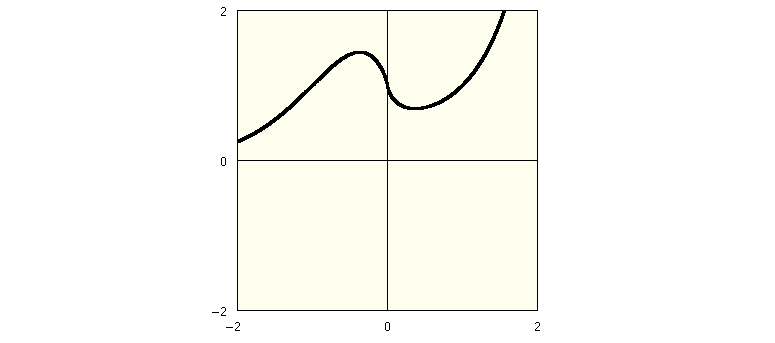
\includegraphics[scale=0.4]{zerozero.png}
\end{center}

\medskip
\noindent
We can see how $0^0=1$ results in a continuous line through $x=0$.
Now let us see how $x^x$ behaves in the complex plane.

\medskip
\verb$f(t)=(real(t^t),imag(t^t))$

\verb$xrange=(-2,2)$

\verb$yrange=(-2,2)$

\verb$trange=(-4,2)$

\verb$draw(f)$

\begin{center}
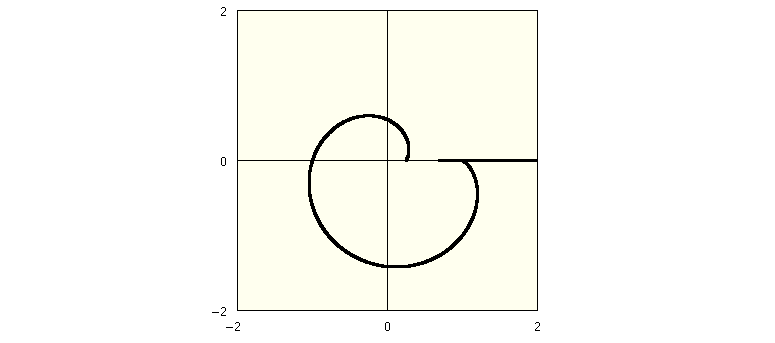
\includegraphics[scale=0.4]{zerozero2.png}
\end{center}
